\section{Experiments} \label{sec:experiments}
Our experiments aim to 
study to what degree entity 
abstraction improves generalization, planning, and modeling.
Sec.~\ref{sec:single_step} shows that from only training to predict how objects fall, OP3 generalizes to solve various novel block stacking tasks with two to three times better accuracy than a state-of-the-art video prediction model. Sec.~\ref{sec:multi_step} shows that OP3 can plan for multiple steps in a difficult multi-object environment. Sec.~\ref{sec:real_world} shows that OP3 learns to ground its abstract entities in objects from real world videos.

\subsection{Combinatorial Generalization without Object Supervision} \label{sec:single_step}

We first investigate how well OP3 can learn object-based representations without additional object supervision, as well as how well OP3's factorized representation can enable combinatorial generalization for scenes with many objects.

\textbf{Domain:} In the MuJoCo~\citep{todorov2012mujoco} block stacking task introduced by~\citet{janner2018reasoning} for the O2P2 model, a block is raised in the air and the model must  predict the steady-state effects of dropping the block on a surface with multiple objects, which implicitly requires modeling the effects of gravity and collisions. The agent is never trained to stack blocks, but is tested on a suite of tasks where it must construct block tower specified by a goal image. \citet{janner2018reasoning} showed that an object-centric model with access to \textit{ground truth} object segmentations can solve these tasks with about 76\% accuracy. We now consider whether OP3 can do better, but \textit{without any supervision on object identity}.


\begin{minipage}{\textwidth}
\begin{minipage}[m]{.39\textwidth}
\footnotesize
    \centering
    \begin{tabular}{ccc}
    \toprule
    SAVP   &  O2P2 &  OP3 (ours)   \\
    \midrule
    24\% & 76\% & \textbf{82\%}\\
    \bottomrule
    \end{tabular}
    \centering
    \captionof{table}{\small{Accuracy (\%) of block tower builds by the SAVP baseline, the O2P2 oracle, and our approach. O2P2 uses image segmentations whereas OP3 uses only raw images as input.}}
    \label{tab:mse_results}
\end{minipage}
 \hfill
\begin{minipage}[m]{.59\textwidth}
\footnotesize
\centering
            \begin{tabular}{c|ccc}
    \toprule
            \# Blocks & SAVP    &  OP3 (xy) & OP3 (entity) \\
         \midrule
              1 & 54\% & 73\% & \textbf{91\%}\\
              2 & 28\%  & 55\% & \textbf{80\%}\\
               3 & 28\%  & 41\% & \textbf{55\%}\\
    \bottomrule
    \end{tabular}
    \centering
    \captionof{table}{\small{Accuracy (\%) of multi-step planning for building block towers. (xy) means \texttt{(pick\_xy, place\_xy)} action space while (entity) means \texttt{(entity\_id, place\_xy)} action space.}}
    \label{tab:multistep_results}
\end{minipage}
\normalsize
\end{minipage}

\textbf{Setup:} We train OP3 on the same dataset and evaluate on the same goal images as~\citet{janner2018reasoning}.
While the training set contains up to five
objects, the test set contains up to nine objects, which are placed in specific structures (bridge, pyramid, etc.) not seen during training.
The actions are optimized using the cross-entropy method (CEM)~\citep{Rubinstein2004TheCM}, with each sampled action evaluated by the greedy cost function described in Sec.~\ref{sec:cost_function}.
Accuracy is evaluated using the metric defined by \citet{janner2018reasoning}, which checks that all blocks are within some threshold error of the goal.

\textbf{Results:} 
The two baselines, SAVP~\citep{lee2018stochastic} and O2P2, represent the state-of-the-art in video prediction and symmetric object-centric planning methods, respectively.
SAVP models objects with a fixed number of convolutional filters and does not process entities symmetrically.
O2P2 does process entities symmetrically, but requires access to ground truth object segmentations.
As shown in Table~\ref{tab:mse_results}, OP3 achieves better accuracy than O2P2, even without any ground truth supervision on object identity, possibly because grounding the entities in the raw image may provide a richer contextual representation than encoding each entity separately without such global context as O2P2 does.
OP3 achieves three times the accuracy of SAVP, which suggests that symmetric modeling of entities is enables the flexibility to transfer knowledge of dynamics of a single object to novel scenes with different configurations heights, color combinations, and numbers of objects than those from the training distribution.
Fig.~\ref{fig:mpc_results} and Fig.~\ref{fig:predicted_components} in the Appendix show that, by grounding its entities in objects of the scene through inference, OP3's predictions isolates only one object at a time without affecting the predictions of other objects.
 
\begin{figure}[!h]
\centering
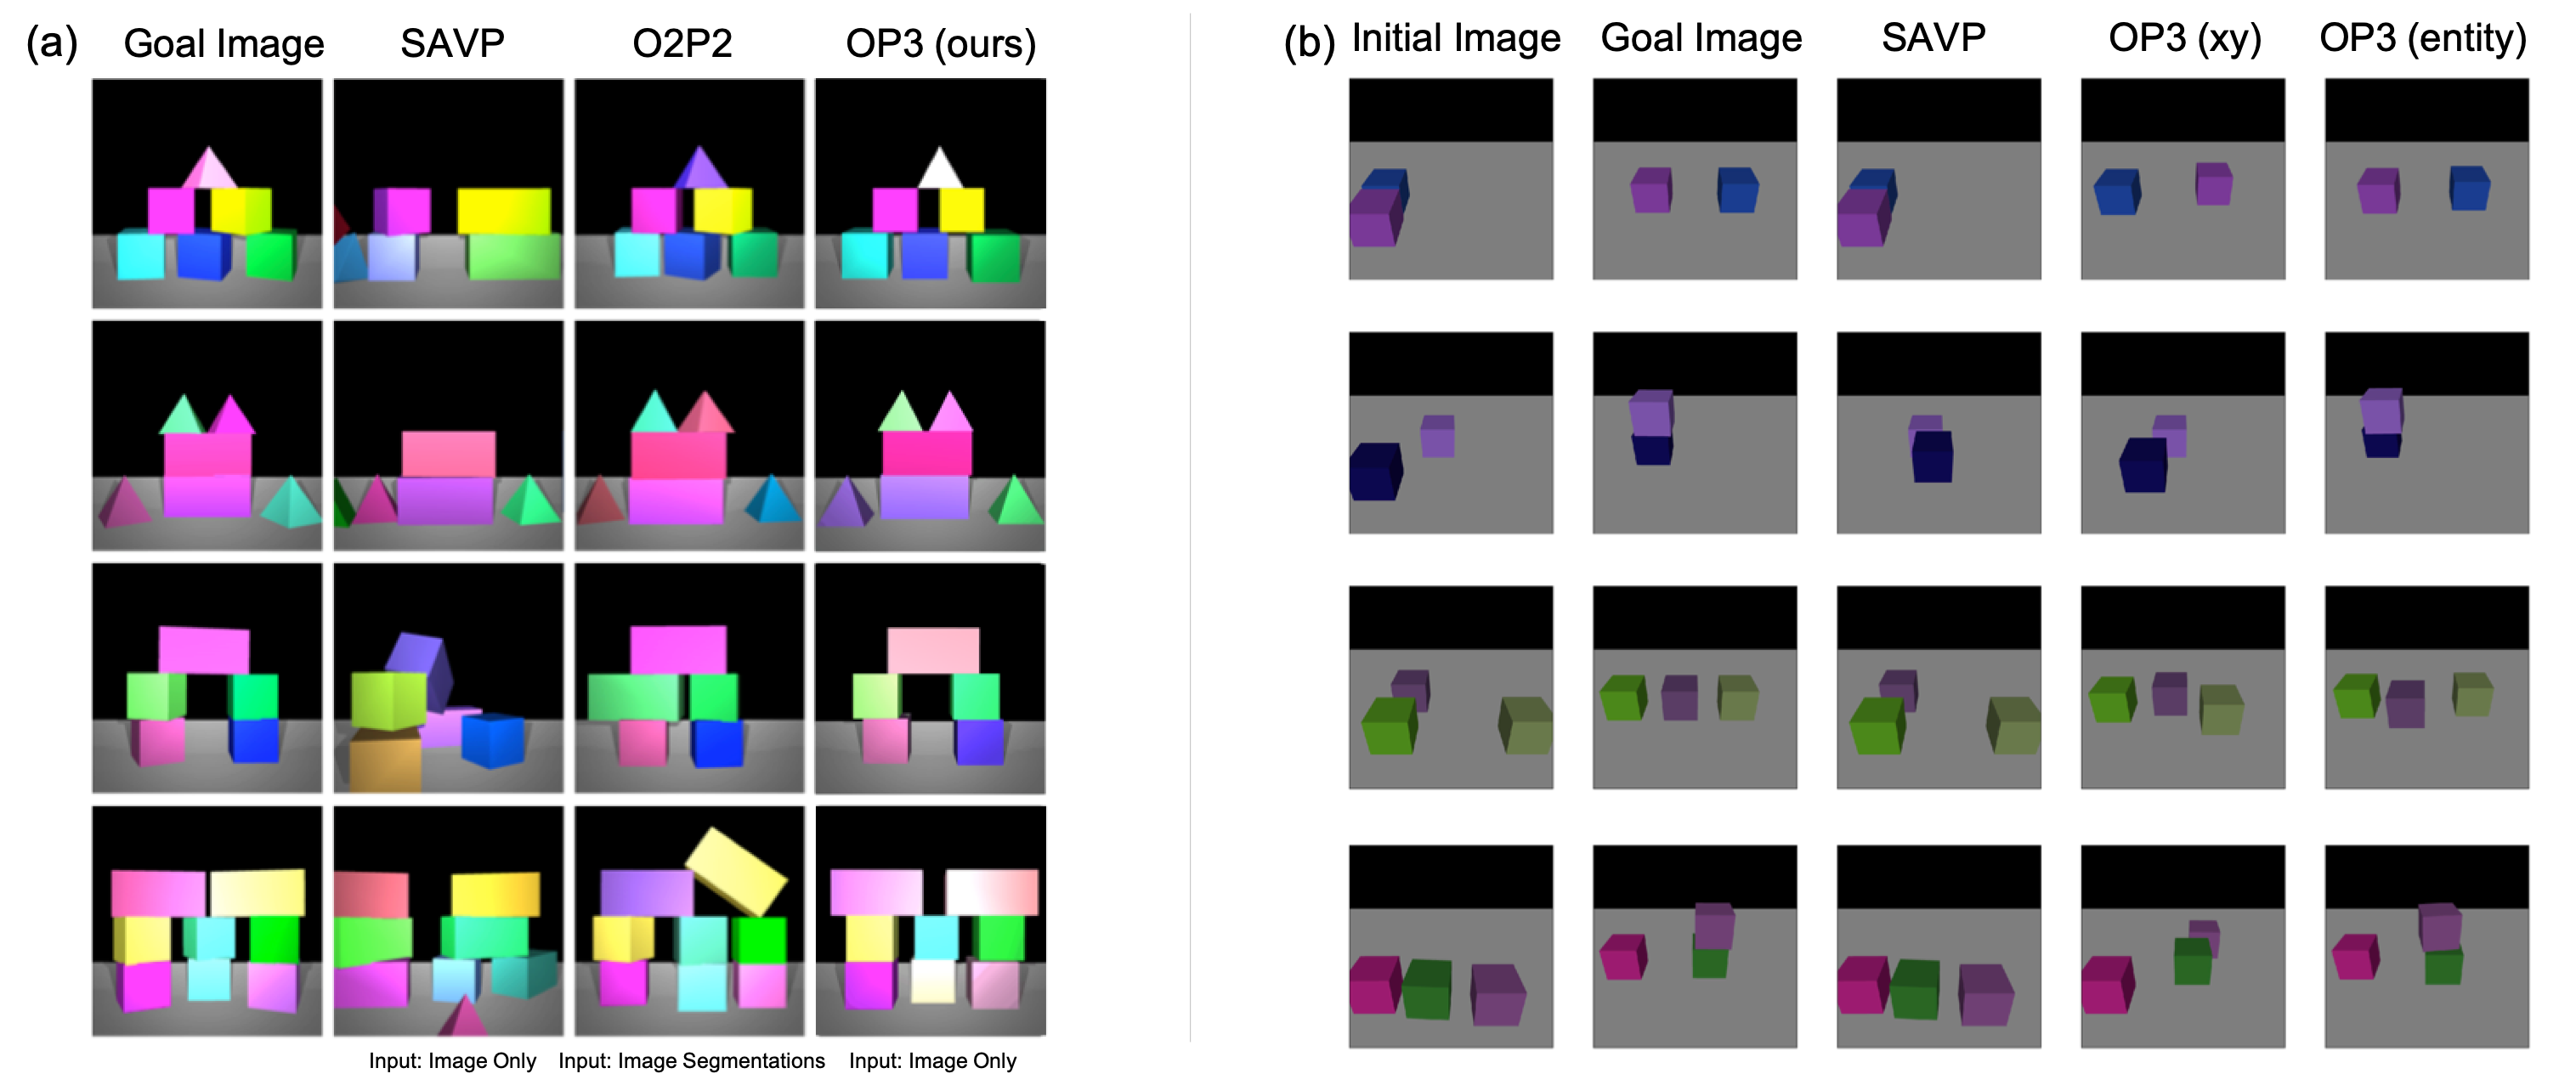
\includegraphics[width=\textwidth]{figs/experiments/stage_1_stage_3.png}
\caption{\small{
\textbf{(a)} In the block stacking task from~\citep{janner2018reasoning} with single-step greedy planning, OP3's generalizes better than both O2P2, an oracle model with access to image segmentations, and SAVP, which does not enforce entity abstraction.
\textbf{(b)} OP3 exhibits better multi-step planning with objects already present in the scene. By planning with MPC using random pick locations (SAVP and OP3 (xy)), the sparsity of objects in the scene make it rare for random pick locations to actually pick the objects. However, because OP3 has access to pointers to the latent entities, we can use these to automatically bias the pick locations to be at the object location, without any supervision (OP3 (entity)).
}}
\label{fig:stage_1_stage_3}
\end{figure}

\subsection{Multi-Step Planning} \label{sec:multi_step}
The goal of our second experiment is to understand how well OP3 can perform multi-step planning by manipulating objects already present in the scene. We modify the block stacking task by changing the action space to represent a picking and dropping location. This requires reasoning over extended action sequences since moving objects out of place may be necessary.

Goals are specified with a goal image, and the initial scene contains all of the blocks needed to build the desired structure. This task is more difficult because the agent may have to move blocks out of the way before placing other ones which would require multi-step planning. Furthermore, an action only successfully picks up a block if it intersects with the block's outline, which makes searching through the combinatorial space of plans a challenge. As stated in Sec.~\ref{sec:planning}, having a pointer to each object enables OP3 to plan in the space of entities.
We compare two different action spaces \texttt{(pick\_xy, place\_xy)} and \texttt{(entity\_id, place\_xy)} to understand how automatically filtering for pick locations at actual locations of objects enables better efficiency and  performance in planning.
Details for determining the \texttt{pick\_xy} from \texttt{entity\_id} are in appendix \ref{appdx:multi_step_block_stacking}.

\textbf{Results:} We compare with SAVP, which uses the \texttt{(pick\_xy, place\_xy)} action space.
With this standard action space (Table \ref{tab:multistep_results}) OP3 achieves between 1.5-2 times the accuracy of SAVP. This performance gap increases to 2-3 times the accuracy when OP3 uses the \texttt{(entity\_id, place\_xy)} action space.
The low performance of SAVP with only two blocks highlights the difficulty of such combinatorial tasks for model-based RL methods, and highlights the both the generalization and localization benefits of a model with entity abstraction.
Fig.~\ref{fig:stage_1_stage_3}b shows that OP3 is able to plan more efficiently, suggesting that OP3 may be a more effective model than SAVP in modeling combinatorial scenes.
Fig.~\ref{fig:interactive_inference_real_world}a shows the execution of interactive inference during training, where OP3 alternates between four refinement steps and one prediction step.
Notice that OP3 infers entity representations that decompose the scene into coherent objects and that entities that do not model objects model the background.
We also observe in the last column ($t=2$) that OP3 predicts the appearance of the green block even though the green block was partially occluded in the previous timestep, which shows its ability to retain information across time.



 \begin{figure}[!h]
\centering
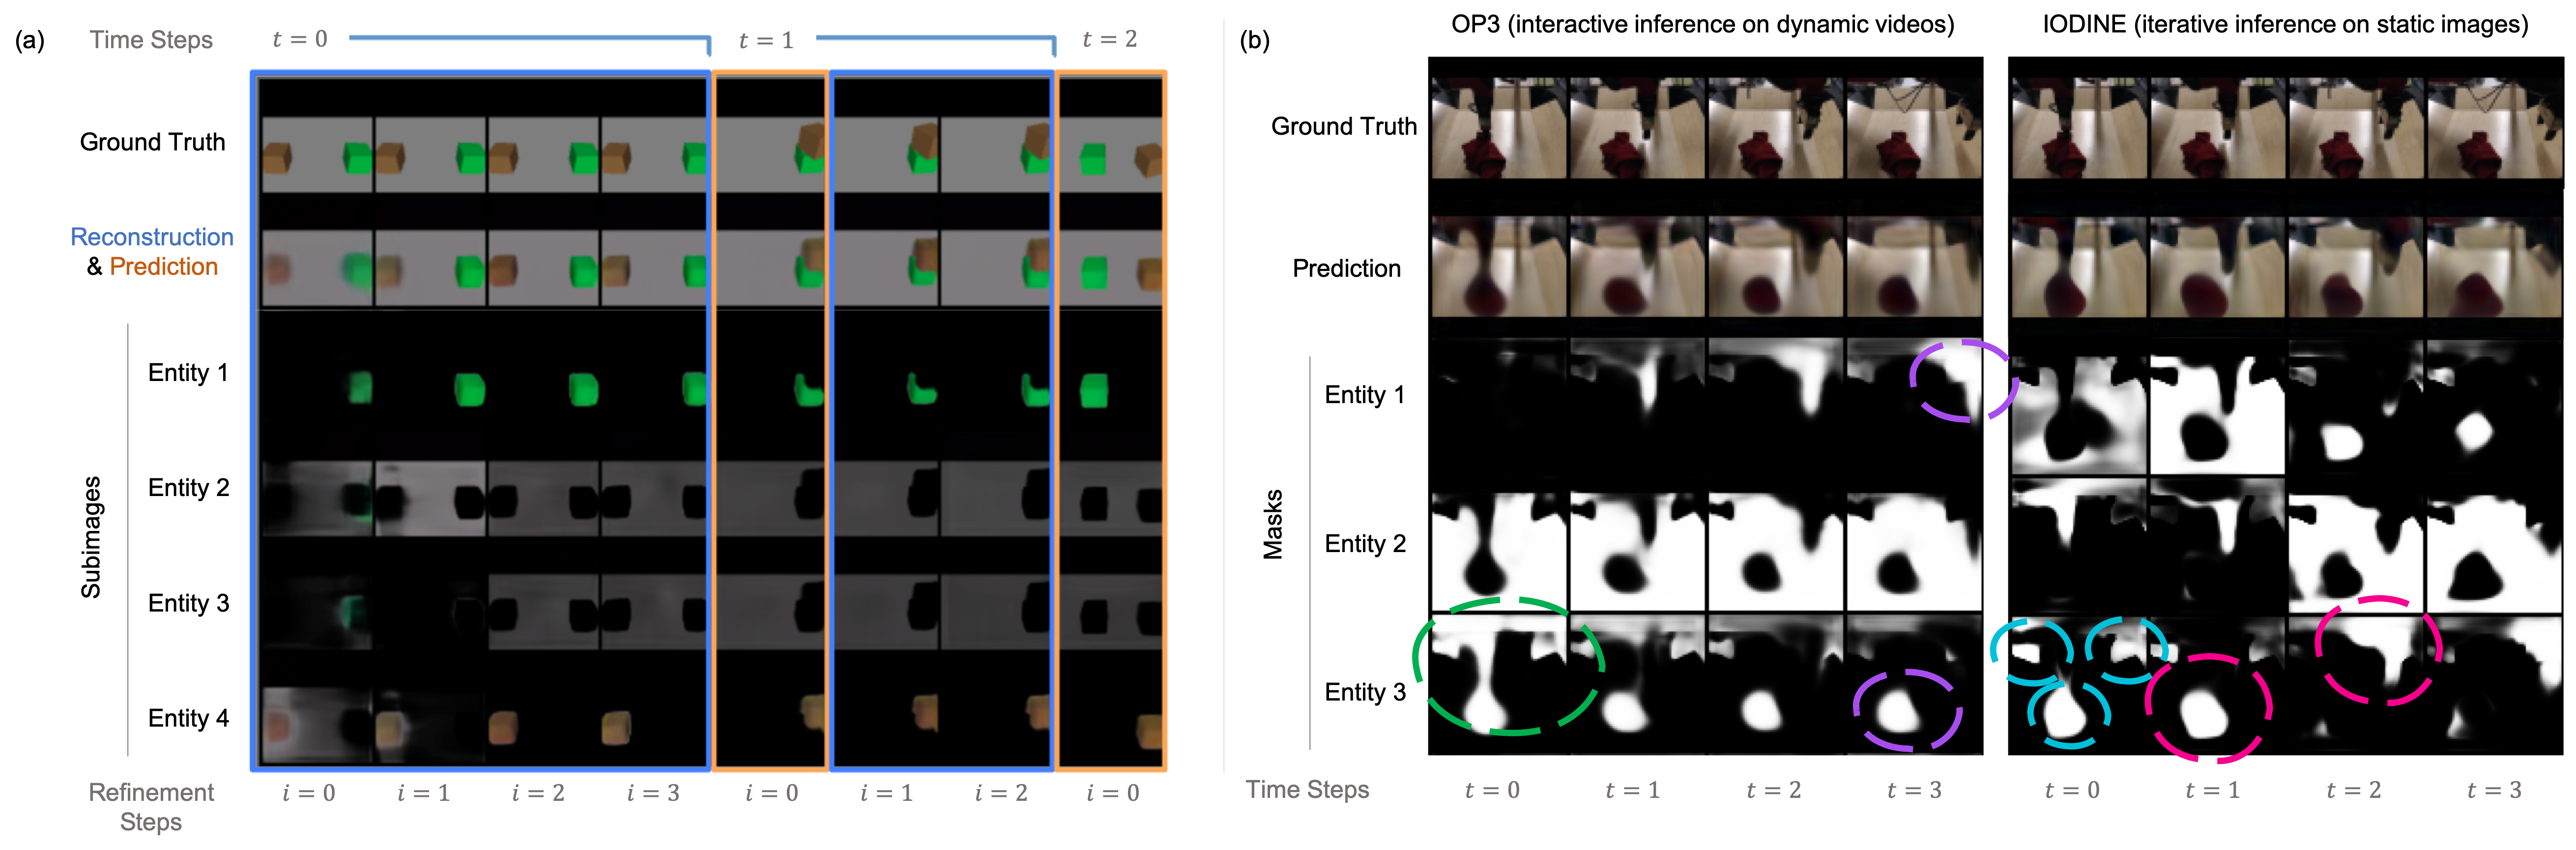
\includegraphics[width=\textwidth]{figs/experiments/interactive_inference_real_world.png}
\caption{\small{
Visualization of interactive inference for block-manipulation and real-world videos~\citep{ebert2018robustness}. Here, OP3 interacts with the objects by executing pre-specified actions in order to disambiguate objects already present in the scene by taking advantage of temporal continuity and receiving feedback from how well its prediction of how an action affects an object compares with the ground truth result.
\textbf{(a)} OP3 does four refinement steps on the first image, and then 2 refinement steps after each prediction.
\textbf{(b)} We compare OP3, applied on dynamic videos, with IODINE, applied independently to each frame of the video, to illustrate that using a dynamics model to propagate information across time enables better object disambiguation. We observe that initially, both OP3 (green circle) and IODINE (cyan circles) both disambiguate objects via color segmentation because color is the only signal in a static image to group pixels. However, we observe that as time progresses, OP3 separates the arm, object, and background into separate latents (purple) by using its currently estimates latents predict the next observation and comparing this prediction with the actually observed next observation. In contrast, applying IODINE on a per-frame basis does not yield benefits of temporal consistency and interactive feedback (red).
}}
\label{fig:interactive_inference_real_world}
\end{figure}


\subsection{Real World Evaluation} \label{sec:real_world}
The previous tasks used simulated environments with monochromatic objects. Now we study how well OP3 scales to real world data with cluttered scenes, object ambiguity, and occlusions. We evaluate OP3 on the dataset from~\citet{ebert2018robustness} which contains videos of a robotic arm moving cloths and other deformable and multipart objects with varying textures.

We evaluate qualitative performance by visualizing the object segmentations and compare against vanilla IODINE, which does not incorporate an interaction-based dynamics model into the inference process. Fig.~\ref{fig:interactive_inference_real_world}b highlights the strength of OP3 in preserving temporal continuity and disambiguating objects in real world scenes. While IODINE can disambiguate monochromatic objects in static images, we observe that it struggles to do more than just color segmentation on more complicated images where movement is required to disambiguate objects.
In contrast, OP3 is able to use temporal information to obtain more accurate segmentations, as seen in Fig.~\ref{fig:interactive_inference_real_world}b where it initially performs color segmentation by grouping the towel, arm, and dark container edges together, and then by observing the effects of moving the arm, separates these entities into different groups.
